%! Author = R2D2 Team 3
%! Date = 14/04/2020

% Preamble
\documentclass[11pt]{article}
\usepackage{hyperref}
\usepackage[official]{eurosym}

\usepackage{graphicx}
\usepackage{tabularx}
\graphicspath{ {./Images/} }

\usepackage{array}

\usepackage{natbib}

\usepackage{xcolor}

\usepackage{color}
\usepackage{colortbl}

\bibliographystyle{apalike}
\renewcommand{\refname}{\section{Referenties}}

\renewcommand{\contentsname}{Inhoudsopgave}

\newenvironment{definition}
    {
        \renewcommand{\arraystretch}{1.2}
        \begin{tabular}{>{\bfseries}l >{\em}p{0.7\textwidth}}
    }
    {
        \end{tabular}
        \renewcommand{\arraystretch}{1}
    }

\newcolumntype{Y}{>{\centering\arraybackslash}X}

\newcommand{\todo}[1]{\textcolor{red}{\emph{#1}}}


\title{Een methode voor pijndetectie door middel van Computer Vision, ge\"{o}rienteerd op embedded systemen}

\author{\emph{R2D2 Team 3} \and Otto de Visser \and Niels Post}

% Document
\begin{document}

    \begin{titlepage}
        \centering
        \maketitle
        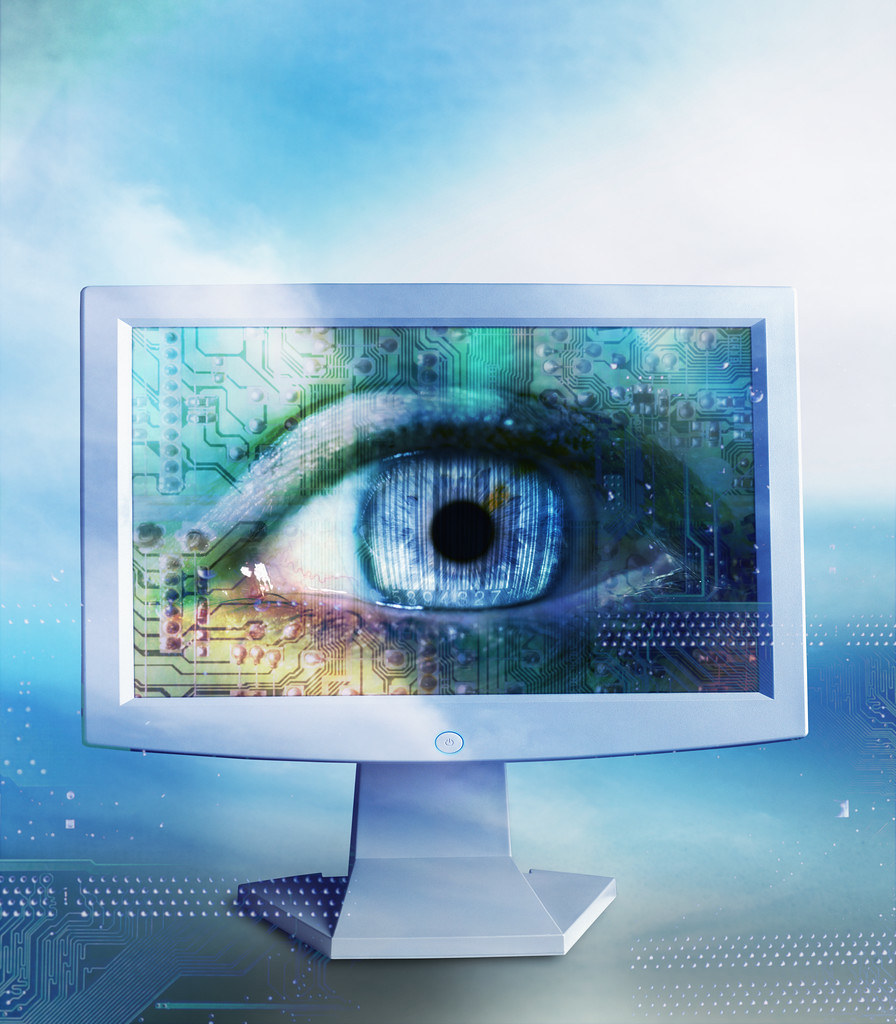
\includegraphics[height=0.6\textheight]{Images/vision.jpg}
        \clearpage
    \end{titlepage}


    \clearpage
    \tableofcontents

    \clearpage


    \section{Abstract}\label{sec:abstract}
    \emph{Work in Progress}
    In dit paper vergelijken wij twee methoden van pijndetectie die werken met Vision.
    Door een literatuuronderzoek stellen wij een basisbegrip van beiden methoden op, en vervolgens vergelijken wij implementaties van de methoden op basis van een aantal vereisten.
    Ook vergelijken wij een set camera's voor algemeen gebruik bij Vision.
    De methode X lijkt beter te zijn omdat Y.
    Camera Z komt als beste uit de test.


    \section{Voorwoord}\label{sec:voorwoord}
    Dit onderzoek wordt uitgevoerd in opdracht van de Hogeschool Utrecht, voor het project R2D2 2020.
    Bij dit project wordt er een ICT-bedrijf gesimuleerd.
    De werkgroep waaronder dit onderzoek valt is Team 3:\\
    \\

    \emph{
        \begin{tabularx}{\textwidth}{YYY}
            Niels Post & Otto de Visser & Amrit Malhi\\
            Menno van der Jagt & Youri de Vor & Finn Fonteijn\\
            Vincent van Setten & Oscar Kromhout
        \end{tabularx}
        \vspace{1em}
    }


    \section{Inleiding}\label{sec:inleiding}

    \emph{R2D2 heeft als bedrijf het doel om multifunctionele, modulaire robots te maken voor gebruik in een rampgebied.
    Omdat in een rampgebied vaak slachtoffers zijn die door allerlei oorzaken hevige pijn hebben,
    is het belangrijk dit te indexeren, en hiernaar prioriteiten te stellen.}

    In dit onderzoek willen wij manieren vinden om door middel van Computer Vision in een klein (embedded) systeem pijnniveaus
    te detecteren.
    Vanwege mogelijke beperkte connectiviteit in een rampgebied onderzoeken wij methoden die volledig automatisch,
    zonder netwerkconnectiviteit of zware hardware kunnen werken.

    Tijdens het lezen van dit onderzoek zal de lezer in de eerste plaats meer leren over vision-algoritmes met pijn
    herkennen als doel.
    Hierbij gaan wij specifiek in op de effici\"{e}ntie, geschiktheid voor embedded systemen, en verwerkingstijden van hardware.
    Hiernaast bespreken wij welke camera's het meest geschikt zijn voor gebruik bij Computer Vision in het algemeen.
    Uiteindelijk kiezen wij 1 combinatie van een algoritme en camera die het best passen bij de context van een pijn
    detectie module binnen een R2D2 robot.


    Om dit onderzoek te defini\"{e}ren zullen wij uit gaan van de volgende onderzoekshoofdvraag:\\

    \begin{definition}
        Hoofdvraag & Welke computer methoden op basis van computer vision zonder gebruik van netwerkconnectiviteit high performance hardware bestaan er waarmee je pijn kan kwantificeren in de context van een embedded systeem?
    \end{definition}


    \bigskip

    Deze hoofdvraag verdelen wij in de volgende 7 deelvragen:

    \begin{enumerate}
        \item\label{itm:dv1} Is het mogelijk om computer vision toe te passen op videobeeld om pijn te kunnen herkennen op het gezicht van een mens?
        \item\label{itm:dv2} Hoeveel foto's per tijdseenheid moeten we minimaal verwerken om zeker te zijn dat we een valide uitspraak kunnen doen over het pijnniveau dat iemand ervaart?
        \item\label{itm:dv3} Wat zijn de minimale hardwarevereisten van een systeem dat pijnmetingen door middel van Computer Vision uitvoert?
        \item\label{itm:dv4} Volgt er een toename in accuraatheid uit het langer analyseren van een frame?
        \item\label{itm:dv5} Wat is de meest geschikte camera voor het toepassen van Computer Vision facial tracking algoritmes met embedded systemen die verkrijgbaar is op de markt?
        \item\label{itm:dv6} Welke bestaande implementaties van een pijnmeting algoritme zijn er, en wat zijn de gebruiksrechten hiervan?
        \item\label{itm:dv7} Wat is de maximaal bereikbare accuraatheid en snelheid bij gebruik van boven onderzochte methoden?
    \end{enumerate}


    \section{Probleemstelling}\label{sec:probleemstelling}
    Voor doktoren is het lastig om een objectief pijn vast te stellen.
    Vaak moet een pati\"{e}nt zelfeen getal tussen de 1 en de 10 geven voor zijn pijn.
    Echter is deze manier van pijn inschatten niet erg objectief, daarnaast is het niet
    altijd mogelijk met de pati\"{e}nt te communiceren.
    In rampscenario's komt het vaak voor dat slachtoffers moeilijk bereikbaar zijn, of dat er niet genoeg dokters zijn om elk slachtoffer apart een dokter toe te sturen.
    Wel is het belangrijk om te weten hoeveel pijn mensen hebben om ze met meer/minder prioriteit te helpen.
    Hierom bestaat de vraag naar een automatische module die pijn detecteert.


    \section{Theorie en hypothese}\label{sec:theorie-en-hypothese}
    De hoofdvraag van dit onderzoek vergelijkt methoden die wij nog niet kennen voor het onderzoek.
    Hierom kunnen wij geen hypothese stellen voor de hoofdvraag.
    Wel kunnen wij een set kleinere hypotheses stellen, betreffende enkele deelvragen.

    \paragraph{\hyperref[itm:dv1]{Deelvraag 1}}
    Van wat wij zelf weten van pijndetectie en herkenning, is dat dit een moeilijk onderwerp is.
    Ondanks dat er universele uitingen van pijn zijn (zoals auw zeggen, en een vertrokken gezicht), is het moeilijk om vast te stellen hoe veel pijn iemand heeft.
    Doktoren vragen hierom dan ook vaak aan mensen om hun pijn een cijfer te geven.\\


    \begin{definition}
        Hypothese & Pijn detecteren met Vision is in algemene zin mogelijk, maar het niveau classificeren is waarschijnlijk lastig of onmogelijk
    \end{definition}

    %    \begin{tabular}{l p{0.7\textwidth}}
    %        \textbf{Hypothese} & \emph{Pijn detecteren met Vision is in algemene zin mogelijk, maar het niveau classificeren is waarschijnlijk lastig of onmogelijk}
    %    \end{tabular}

    \paragraph{\hyperref[itm:dv3]{Deelvraag 3}}
    Wij verwachten dat de belangrijkste vereiste van een systeem een minimale hoeveelheid werkgeheugen is.
    Omdat er geen directe deadline is voor een berekening, kan een processor hier langer over doen, maar als het geheugen niet toereikend is, kan een afbeelding niet opgeslagen worden voor verwerking.

    Microcontrollers hebben vaak weinig (minder dan 100kB) werkgeheugen.
    Het bijplaatsen van geheugen is maar beperkt mogelijk.
    Een limiterende factor heirvoor is namelijk dat microcontrollers vaak een 16 bits processor hebben, en deze niet meer dan +- 131 kB aan geheugen kunnen adresseren.
    Hierom verwachten wij dat de meeste microcontrollers geen effectieve Vision algoritmes kunnen draaien.
    Hiermee bedoelen we dat het uitvoeren van Vision algoritmen wel mogelijk is, maar dat deze niet op een zodanige kwaliteit (resolutie) uitgevoerd kunnen worden dat het resultaat accuraat is.


    \begin{definition}
        Hypothese & Voor een Vision-gebaseerd pijnmetingsalgoritme is een embedded systeem nodig wat minimaal een 32 bits processor heeft.
    \end{definition}

    \paragraph{\hyperref[itm:dv4]{Deelvraag 4}}
    Wij zijn tot nu toe via lessen bij het vak Computer Vision in aanraking geweest met een aantal Computer Vision algoritmes.
    Een deel hiervan hebben wij zelf uitgewerkt in de huiswerkopdracht gezichtsdetectie, en een deel hebben wij alleen in theorie kort behandeld.
    Bij deze algoritmes , was de uitkomst steeds gebaseerd op een vaste set handelingen.
    Omdat deze handelingen niet afhankelijk zijn van entropie, was het resultaat altijd hetzelfde.
    Wij denken dat de handelingen voor pijndetectie op dezelfde manier zullen werken, aangezien deze ook te maken zullen hebben met het detecteren van gezichtskenmerken.\\

    \begin{definition}
        Hypothese & Het langer analyseren van een videoframe zal geen accuratere resultaten geven bij een pijnmetingsalgoritme op basis van computer vision
    \end{definition}

    \paragraph{\hyperref[itm:dv5]{Deelvraag 5}}
    Computer Vision algoritmes zijn hevig afhankelijk van detectie van kleuren, contrasten en randen.
    Omdat de verwerking hiervan afhankelijk zijn van het kleurpalet van de gebruikte camera, denken wij dat er camera's zullen zijn die specifiek gericht zijn op Computer Vision.
    Mogelijk gebruiken deze camera's geen RGB, maar een uitgebreider kleurenschema, zoals bijvoorbeeld ARGB.\\

    \begin{definition}
        Hypothese & Er zijn camera's op de markt beschikbaar die specifiek gericht zijn op Computer Vision algoritmes.
    \end{definition}


    \section{Begrippenlijst}\label{sec:begrippenlijst}

    \begin{definition}
        Computer Vision & Een algemene term voor algoritmes die gebruik maken van camerabeelden, en hier conclusies uit trekken\\

    \end{definition}


    \section{Uitvoering}\label{sec:uitvoering}

    \subsection{Deelvraag 1 tot en met deelvraag 4}\label{subsec:deelvraag-1-tot-en-met-deelvraag-4}
    Voor deze deelvragen zullen wij een literatuuronderzoek
    verrichten naar methoden van pijndetectie door middel van Vision.
    Hierbij zullen wij per methode de deelvragen beantwoorden, om zo uiteindelijk een conclusie te kunnen trekken over
    de meest geschikte methode(n).
    Voor het aangeven van de hardware-vereisten maken wij een beredenering waarom wij denken dat er een bepaalde hardware-vereiste is.
    In deze beredenering kijken we vooral naar het geheugengebruik van de methode,
    aangezien dit de meest limiterende factor is van een embedded systeem.

    Om de onderzochte methoden inzichtelijk te maken voor onszelf, beantwoorden wij voor onszelf een aantal vragen over elke methode.
    Omdat de antwoorden op deze vragen niet direct relateren aan de deelvragen, maar een methode inzichtelijk dienen te maken, kan de lezer de antwoorden hierop vinden inde bijlagen.
    Deze vragen zijn als volgt:
    \begin{itemize}
        \item Korte Omschrijving
        \item Van welk principe maakt het gebruik
        \item Geschatte piek-geheugengebruik per meting
        \item Geschatte tijdsduur voor een conclusie
        \item Mogelijkheid om te draaien op een embedded systeem
    \end{itemize}


    Voor \emph{\hyperref[itm:dv1]{deelvraag 5}} doen wij een vergelijkend onderzoek voor camera's.
    We onderzoeken het bestaan van camera's specifiek voor vision, en noteren specificaties van deze camera's.
    Bij dit onderzoek betrekken wij ook een webcam en een actiecamera.
    In dit onderzoek bepalen wij een aantal attributen die de camera moet/mag hebben voor werking bij computer vision op een embedded systeem.
    Volgens deze attributen maken wij een vergelijking van de camera's.

    Voor deelvraag 6 doen wij experimenteel onderzoek.
    Door meerdere implementaties te vergelijken, kunnen wij de maximale bereikbare waarden ervan vergelijken.


    \section{Resultaten}\label{sec:resultaten}

    \subsection{Deelvraag 1 t/m 4}\label{subsec:deelvraag-1-t/m-4}
    \emph{Is het mogelijk om computer vision toe te passen op videobeeld om pijn te kunnen herkennen op het gezicht van een mens?}

    Wij hebben een aantal velden opgesteld die wij per methode hebben onderzocht.
    De volgende resultaten zijn hieruit gekomen

    \subsubsection{Methode 1: Facial Feature detection}
    \emph{\citet{werner2014automatic}} Automatic pain recognition from video and biomedical signals\\
    \emph{\citet{prkachin1992consistency}} The consistency of facial expressions of pain: a comparison across modalities\\
    Deze methode combineert het gebruik van Vision algoritmen, met het meten van biomedische data door middel van sensoren.
    Omdat dit onderzoek Vision beschrijft, zullen wij het sensoraspect van dit onderzoek niet verwerken. In plaats daarvan gaan we dieper in op de referenties gemaakt in het paper met betrekking tot Vision.

    \paragraph{Aantal foto's per tijdseenheid}
    Deze methode maakt gebruik van veranderingen in gezichtsafstanden ten opzichte van een baseline, en kan dus met 2 foto's een resultaat geven.
    Deze foto's hoeven dan ook niet extreem snel verwerkt te worden, en het systeem mag hier een aantal seconden over doen.

    \paragraph{Hardware-vereisten}\label{meth1-hardware}
    De vereisten voor de berekening zelf zijn weinig: Er moeten slechts een aantal afstanden van coordinaten vergeleken worden.
    Dit zullen de meeste microcontrollers ook kunnen.
    Het probleem zit hierom meer in de methode van facial feature detection.
    Afhankelijk van de gebruikte methode, moet de processor mogelijk meerdere kleurafbeeldingen opslaan, en bij convolutie van een afbeelding moet een afbeelding vaak twee keer aanwezig zijn in het geheugen.

    \emph{Bij de onderstaande redenering gaan wij uit van onze ervaring in algemene gezichtsdetectie, aangezien wij geen diepgaande ervaring hebben met gezichtseigenschappen-detectie.
    Mogelijk is zo een algoritme dus meer/minder geheugenintensief dan wij aannemen}

    Bij het opslaan van een kleine kleurafbeelding (50x50) is al gauw 7.5KB per afbeelding nodig. (2500 pixels van 3 bytes (rgb))
    Omdat naast een aantal van deze afbeeldingen en eventuele afbeeldingsbuffers ook nog de programmacode aanwezig moet zijn op de microcontroller,
    verwachten wij dat dat deze methode niet zal kunnen draaien op een standaard microcontroller.


    Mogelijk zijn uitgebreidere microcontrollers wel toereikend.
    Een Arduino Due heeft bijvoorbeeld 96kB werkgeheugen.
    De marge vinden wij hier echter te klein van.
    Bij het toevoegen van meer functionaliteit zou ook het geheugen van een Due snel volraken.
    Om deze reden raden wij aan om deze methode te draaien op een embedded systeem met werkgeheugen op het circuitboard.
    Denk hierbij aan een Raspberry Pi of een Nvidia Jetson-systeem

    \paragraph{Langer analyseren frame}
    Of pijn accurater gedetecteerd kan worden is grotendeels afhankelijk van de gebruikte methode voor facial feature recognition.
    Het langer analyseren kan wel effect hebben op de afstand waarop pijn gedetecteerd kan worden.
    Dit zou mogelijk zijn door de afbeelding op volledige resolutie te verwerken, en niet omlaag te schalen.

    \subsubsection{Methode 2: Optical Flow}
    \emph{\citet{werner2014automatic}} Automatic pain recognition from video and biomedical signals\\
    \emph{\citet{prkachin1992consistency}} The consistency of facial expressions of pain: a comparison across modalities\\
    Deze methode combineert het gebruik van Vision algoritmen, met het meten van biomedische data door middel van sensoren.
    Omdat dit onderzoek Vision beschrijft, zullen wij het sensoraspect van dit onderzoek niet verwerken. In plaats daarvan gaan we dieper in op de referenties gemaakt in het paper met betrekking tot Vision.

    \paragraph{Aantal foto's per tijdseenheid}

    \paragraph{Hardware-vereisten}

    \emph{Bij de onderstaande redenering gaan wij uit van onze ervaring in algemene gezichtsdetectie, aangezien wij geen diepgaande ervaring hebben met gezichtseigenschappen-detectie.}

    \paragraph{Langer analyseren frame}

    \subsection{Deelvraag 5 }\label{subsec:deelvraag-5}
    \emph{Wat is de meest geschikte camera voor het toepassen van Computer Vision facial tracking algoritmes met embedded systemen die verkrijgbaar is op de markt?}

    Bij het vergelijken van de camera's gebruiken wij de volgende attributen.

    \vspace{1em}

    \noindent \underline{Resolutie: Minimale resolutie van 50px*50px} \hfill Must have\\
    Deze resolutie is minimaal om accurate resultaten te krijgen met Vision\footnote{Zoals beschreven in \citet{boom2006effect}}

    \noindent \underline{Stroomverbruik: Minder dan 1 W stroomverbruik} \hfill Must have\\
    Er is op een los bewegende robot geen grote stroombron aanwezig om een camera continu aan te sturen.

    \noindent \underline{Universeel: Universele aansluiting} \hfill Should have\\
    De camera moet op een standaarplatform kunnen draaien, zodat er geen converters/chips aan het systeem toegevoegd moeten worden

    \noindent \underline{Lichtgewicht: lichter dan 300g} \hfill Should have\\
    De camera moet gedragen kunnen worden door een R2D2 robot

    \noindent \underline{Formaat: kleiner dan 10x5x5cm} \hfill Should have\\
    De camera moet niet groter zijn dan het board wat hem aanstuurt, zo houden we de module klein

    \noindent \underline{Vision: Kan zelf gezichtstracking uitvoeren} \hfill Could have\\
    Als de camera zelf facial tracking technieken kan uitvoeren, kunnen wij de hardware-vereisten van de verbonden microcontroller beperken

    \noindent \underline{Monteren: Met montagebeugel of soortgelijk} \hfill Could have\\
    Als de camera geleverd wordt met een makkelijke manier om hem te bevestigen, kan deze ook makkelijk op een R2D2 robot bevestigd worden


    \vspace{1em}

    We vergelijken de volgende camera's

    \paragraph{Pixy2}
    \href{https://pixycam.com/pixy2/}
    De pixy2 is een camera die specifiek gericht is op het gebruiken van Vision algoritmes in microcontrollers.
    Deze camera heeft veel ondersteunde communicatiemethoden die gebruikt kunnen worden met microcontrollers en embedded systemen.
    De camera heeft zelf een chip die lijnen, kleuren en specifieke objecten kan herkennen.
    Hiernaast kan via USB ook een live camerabeeld uitgelezen worden.


    \emph{Attributen verzameld via [\citenum{pixy_datasheet}]}

    \paragraph{Flir Firefly DL}
    \href{https://www.flir.com/products/firefly-dl/}
    De firefly DL is een Specifieke Computer Vision camera, gericht op vision door middel van Deep Learning.
    Dit is een camera die aangesloten kan worden op een computer om een neural network te trainen voor een bepaald doel.
    Hierna kan het getrainde netwerk geladen worden op de camera, die vervolgens via een USB verbinding de resultaten en het beeld kan doorsturen.


    \emph{Attributen verzameld via [\citenum{firefly_info}]}

    \paragraph{Webcam: Logitech C270}
    De makkelijkst verkrijgbare camera is natuurlijk een webcam. Deze doet niks voor ons in de vorm van Vision, en levert alleen beelden.
    Wel heeft deze een hele toegankelijke interface (USB2) die op veel embedded systemen beschikbaar is.

    \emph{Attributen verzameld via [\citenum{c270_datasheet}]}


    \scriptsize{
    \makebox[0.9\textwidth]{
        \begin{tabular}{l|c|c|c|c|c|c|c}
            \textbf{Camera} & \textbf{Resolutie} & \textbf{Stroomverbruik} & \textbf{Universeel} & \textbf{Lichtgewicht} & \textbf{Formaat} & \textbf{Vision} & \textbf{Monteren}\\
            \hline
            Pixy2 & 1296x976 & 0.495W  & SPI/I2C/UART/USB & 10g & 4.2x3.8x15 cm & Alleen Object tracking & Schroefgaten\\
            Firefly & 1440x1080 & 2.2W &USB 3.1 & 20g & 2.7x2.7x1.45 cm & Divers.\footnotemark[1] & getapte gaten\\
            C270 & 1280 x 720 & onbekend & USB & 226g & 7 x 3.1 x 2.1 \footnotemark[2] cm & Geen & Klemsysteem\\
        \end{tabular}
    }
    }
    \footnotetext[1]{Op een computer wordt een neural network getraind, wat geladen kan worden op de camera}
    \footnotetext[2]{Afmetingen uit het datasheet leken niet te kloppen, dus wij hebben dit handmatig opgemeten}



    \section{Conclusie en Discussie}\label{sec:conclusie-en-discussie}
    \emph{Work in Progress}
    \subsection{Vergelijking algoritmen}
    Op het moment van schrijven zijn wij nog niet begonnen met de implementatie.



    De indruk die opgewekt is in dit literatuur onderzoek is dat deze methode complex is in implementatie en eigenlijk niet perfect onze vereisten vervult.
    Onder andere zijn dus meerdere frames van de transistie tussen neutraal en een een expressie nodig om te kunnen vast stellen welke expressie dit is.
    Alhoewel optical flow technieken goed werken op lage resolutie beelden moeten deze beelden verder van hoge kwaliteit zijn.
    Ook dit is een min punt van deze aanpak.

    \subsection{Vergelijking camera's}
    Voor de vergelijking van camera's zijn we het erover eens dat voor gebruik bij computer vision de Firefly-DL de meest geschikte camera is.
    Door de Deep Learning mogelijkheden kan een algoritme dat gezichtskenmerken detecteert veel aangepast worden om precieze resultaten te leveren.
    Deze camera is echter minder geschikt voor embedded systemen door het hogere stroomverbruik en minder bruikbare interface.
    Er zijn namelijk weinig embedded systemen met een USB 3.1 aansluiting\footnotemark[3]

    \footnotetext[3]{Mogelijk werkt de camera wel met USB 2, maar hier konden wij niks over vinden in de gegevens, en wij konden dit niet testen zonder de camera}

    De Pixy2 is op dit vlak geschikter, aangezien de interfacemogelijkheden specifiek gericht zijn op embedded systemen.
    De Pixy voegt echter binnen de scope weinig toe voor gezichtskenmerk-tracking, aangezien het alleen vooraf bekende objecten/kleuren kan herkennen.

    Om niet meer functionaliteit te kopen dan nodig is, is daarom onze keuze gevallen op de standaard webcam.
    Doordat de camera zelf geen Vision mogelijkheden heeft, zal er een sterker embedded systeem nodig zijn \hyperref[meth1-hardware]{(zie hardware-vereisten)} om de algoritmen uit te voeren.
    Een groot voordeel, zeker in coronatijd is dat de meeste mensen wel een webcam thuis hebben staan, en de resultaten van dit onderzoek daarom goed reproduceerbaar zijn.


    \section{Evaluatie}\label{sec:evaluatie2}
    \emph{Work in Progress}
    Vanwege meerdere minpunten met als belangrijk dat relatieve verschillen gemeten kunnen worden raden we niet aan om deze methode te gebruiken voor ons doeleinde.


    \section{Aanbevelingen}\label{sec:aanbevelingen2}
    \emph{Work in Progress}
    Onze aanbeveling is om deze methode niet te gebruiken voor pijn detectie en door te zoeken naar een andere, effectievere methode.



    \section{Suggesties voor verder onderzoek}\label{sec:suggesties-voor-verder-onderzoek2}
    \emph{Work in Progress}
    Er is nog veel te lezen over optical flow methodes en hoe je deze effectief implementeert.
    Er is een \emph{\citet{Readinglist} Reading list}.
    Hier staan op dit moment 72 artikels in over optical flow technieken.

    \paragraph{Pixy2}
    Ondanks dat de pixy camera geen gezichtskenmerken kan herkennen, is het misschien wel mogelijk om een algoritme efficienter te laten werken door de pixy voorwerk te laten doen.
    Er kan onderzocht worden of het mogelijk is met de Pixy om oninteressante gebieden uit te sluiten van berekening in een algoritme.
    Hierdoor kunnen algoritmen mogelijk op minder sterke microcontrollers uitgevoerd worden, of sneller resultaten leveren.


    \section{Literatuur}\label{sec:literatuur2}
    \emph{Work in Progress}
    In dit hoofdstuk beschrijven we de onderzochte literatuur.
    Hierbij geven wij aan wat de relevantie is tot ons eigen onderzoek.


    \section{Bijlagen}\label{sec:bijlagen}

    \subsection{Invullingen onderzoek}\label{subsec:invullingen-onderzoek}

    \subsubsection{Invulvelden}
    In het volgende onderdeel beschrijven wij per methode de antwoorden op deze invulvelden.
    Hierbij interpreteren wij resultaten, en trekken conclusies.
    Deze resultaten hoeven dus niet direct uit het onderzoek overgenomen te zijn.

    \subsubsection{Methode 1}
    Deze methode is gebaseerd op het onderzoek (\citet{werner2014automatic}).
    Deze methode beschrijft pijndetectie door middel van het interpreteren van de afstand tussen specifieke gezichtskenmerken.

    \paragraph{Korte Omschrijving}
    Het paper omschrijft een bredere methode, maar wij leggen de focus op het gedeelte vision.
    Deze methode detecteert pijn door te kijken naar de positie van bepaalde gezichtseigenschappen ten opzichte van elkaar.
    Zo kan pijn zich bijvoorbeeld uiten in een "samengetrokken" gezicht.

    \paragraph{Van welk principe maakt het gebruik?}
    Relationele positie van gezichtseigenschappen

    \paragraph{Geschatte piek-geheugengebruik per meting}
    Wij gaan uit van een ruime minimum voor gezichtsdetectie.
    Gezichtsdetectie en herkenning functioneren beduidend minder onder een resolutie van 50x50 pixels zoals beschreven in \citet{boom2006effect}.
    Hier gaan wij dan ook vanuit bij het geheugengebruik.
    Een afbeelding van 50x50 gebruikt +- 7.5kB in ruimte.

    Methoden van facedetection zijn ons niet bekend, hierom is dit moeilijk in te schatten.
    Ervanuitgaande dat er convolutie-operaties uitgevoerd worden op de afbeelding zal de afbeelding hoogst waarschijnlijk op momenten meerdere keren in het geheugen moeten bestaand.
    Hiernaast moet de draaiende programmacode, en eventuele image kernels toegevoegd worden.
    In piek zal dit programma minimaal 50 kB geheugen gebruiken, maar naar alle waarschijnlijkheid meer.

    \paragraph{Geschatte tijdsduur voor 1 conclusie}
    Wij denken dat er minimaal 2 metingen gedaan moeten worden.
    Dit omdat het gezicht vergeleken moet worden, en de samentrekking van het gezicht ten opzichte van de eerste meting bepaald moet worden.

    Op een adequate computer hoeft een meting niet veel langer te duren dan 0,1 seconde.
    Twee metingen zouden dan zo'n 0.2 seconden duren.

    \paragraph{Embedded capaciteit}
    Zoals wij al enigszins hadden verwacht is het niet redelijkerwijs mogelijk dit te draaien op een Arduino.
    Dit is voornamelijk omdat het piek-geheugengebruik te groot is hiervoor.
    Wel is dit prima mogelijk om te draaien op een Raspberry Pi of een mini-pc.

    \paragraph{Maximale geschatte effectieve afstand}
    Dit is voornamelijk afhankelijk van de tijd die wij besteden aan het herkennen.
    In combinatie met een camera met een hoge resolutie kunnen afstanden van vele meters gehaald worden (uitgaande van een minimum gezichtsgrootte van 50pxx50px.
    Hiervoor zou een face detection algoritme wel erg vaak/erg precies uitgevoerd worden, wat de verwerkingstijd flink vergroot.
    De maximale afstand is in dit geval dus afhankelijk van de maximale verwerkingstijd

    \paragraph{Kosten vereiste specifieke apparatuur}
    Voor deze methode is alleen een (mini)-pc en een camera vereist.
    Een (minimale) combinatie van een Raspberry Pi (\euro{}40) en een standaard webcam(\euro{}30) zou ongeveer \euro{}70,- kosten.

    \paragraph{Haalbaarheid}
    Wij denken dat deze methode voor onze scope haalbaar is, met een paar aanpassingen:
    \begin{itemize}
        \item Deze methode projecteert gezichtseigenschappen op een 3d-model van een gezicht.
        Hier hebben wij noch ervaring, noch tijd voor om uit te werken.
        Om dit te vermijden zouden wij de aanname doen dat iemand recht in de camera kijkt.
        Zo kunnen wij toch met zekerheid afstanden tussen gezichtseigenschappen meten.
        \item Zoals eerder aangegeven richten wij ons enkel op het vision-gedeelte van dit onderzoek, niet op de biomedische sensoren.
    \end{itemize}

    \paragraph{Mogelijke implementatie}
    Wij maken gebruik van DLib, een c++ library waar een methode voor facial feature detection in opgenomen is.
    Uit een eerste foto/meting extraheren wij een aantal afstanden tussen bepaalde gezichtskenmerken, en slaan deze op.
    Hierna doen wij steeds opnieuw metingen en vergelijken dit met de oorspronkelijke afstandsmetingen,
    hierbij kijkend naar de specifieke veranderingen zoals genoteerd in de onderzochte papers.

    \subsubsection{Methode 2}

    \emph{\citet{barronperformance} Performance Of Optical Flow Techniques.}\\ \\
    \emph{\citet{naghsh2006efficient} An Efficient Algorithm for Motion Detection Based Facial Expression Recognition using Optical Flow.}\\ \\
    \emph{\citet{zainudinfacialexpression} Facial expression change detection algorithm using optical flow technique.}\\ \\

    \paragraph{Korte Omschrijving}
    Methode 2 draait om de zogenoemde techniek optical flow.
    Dit is een veel gebruikte techniek om verandering tussen frame in beeld te brengen en te kwantificeren.

    \paragraph{Van welk principe maakt het gebruik?}
    Deze techniek kijkt naar verschillen tussen frames en probeert de richting van verandering vast te stellen.
    De stappen die uitgevoerd worden zijn alsvolgd:
    1. Er wordt een frame gebufferd.
    2. Er wordt een tweede frame gebufferd.
    3. Voor elke pixel in de eerste frame wordt in de tweede frame gekeken of deze kleur en intensiteit ongeveer te vinden is in de buurt van de oorspronkelijke pixel in de eerste frame.
    4. Op deze manier breng je beweging van pixels tussen frames in beeld.
    5. Vaak zijn er ook passes met grotere bins van 2

    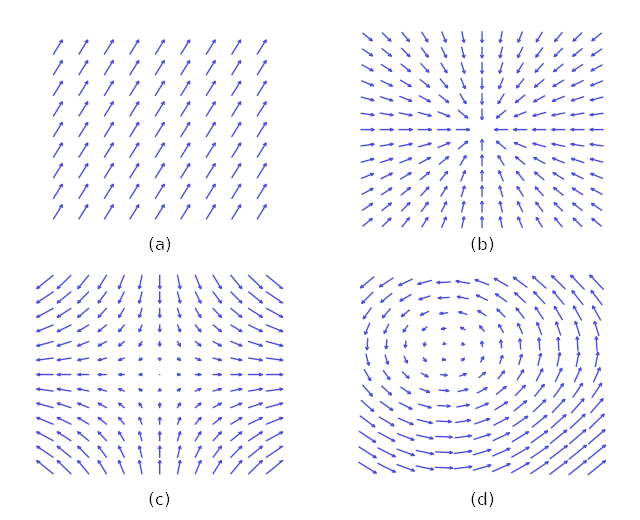
\includegraphics[height=0.2\textheight]{Images/Vector-field-examples.jpg}
    Er wordt over het gezicht gekeken naar verandering, welke uitgedrukt worden in vectoren.
    Deze worden dan gematcht tegen een database met de verschillende emoties.
    Door dat je verandering in mensen hun gezicht registreerd/

    \paragraph{Geschatte piek-geheugengebruik per meting}
    Gezien de ondergrens 3 frames is voor enige nauwkurigheid zijn de geheugen eisen voor het bewaren van de frames niet groot.

    \paragraph{Geschatte tijdsduur voor 1 conclusie}
    De techniek kan met drie frames al een nauwkurigheid van 83\% opleveren volgens \emph{\citet{naghsh2006efficient}}.
    Deze drie frames zouden echter wel de verschillende staten van de emotie die uitgedrukt worden moeten in beeld moeten brengen.
    De geschatte tijdsduur zal dan ook grote deels afhankelijk zijn van de tijd die het kost om deze frames te verzamen.
    De analysetijd is echter wel relatief lang, niet in de buurt van real time op een embedded systeem, echter is dit geen requirement en dus geen probleem.

    \paragraph{Embedded capaciteit}
    De berekening die uitgevoerd moeten worden zijn een heleboel relatief simpele operaties.
    Een embedded systeem zou hier relatief lang over doen (seconden), maar het is zeker niet onmogelijk.
    De precieze capaciteiten moeten worden vast gesteld met testen maar we hebben vertrouwen dat het mogelijk is om deze module te draaien op een Raspberry Pi.

    \paragraph{Maximale geschatte effectieve afstand}
    Je hebt geen hoge resolutie nodig om de gezichtseigenschappen te kunnen traceren met optical flow.
    Om deze methode goed uit te kunnen voeren op een embedded systeem wil je bij voorkeur een volledig gezicht zonder achtergrond.
    Om dit voor elkaar te krijgen zou je moeten het gezicht moeten uitvergroten.
    Op lage kwaliteit cameras levert dit meer ruis op, wat problemen levert in optical flow berekening.
    De benodigde berekeningen kunnen tot ongeveer 200x200 pixels uitgevoerd worden en met een standaard wide angle camera zou dit tot enkele meters haalbaar moeten zijn.

    \paragraph{Kosten vereiste specifieke apparatuur}
    We hebben hiervoor een camera (20 euro) en Raspberry Pi minimaal model 3B+ (35 euro), maar liever een model 4B (40 euro).

    \paragraph{Haalbaarheid}
    Wij zijn twijfelachtig over de werkelijke Haalbaarheid van deze methode, gezien de complexiteit van implementatie.
    Het zou haalbaar moeten zijn als we een paar voorwaarden hebben:
    \begin{itemize}
        \item Goed belichte, hoog contrast en laag ruis input beeld.
        \item In het input beeld alleen het gezicht met gezichtseigenschappen al getagt.
    \end{itemize}

    \paragraph{Mogelijke implementatie}
    Een mogelijke implementatie zou berusten op enige bestaande libaries zoals libd of opencv.
    Dit omdat de implementatie van deze methode complex is en we het werk dat wij moeten doen zo veel mogelijk willen inperken tot wat nog niet bestaat.
    Dubbel werk doen is nooit handig, en al helemaal niet als het werk dat je wel moet doen zo complex is.


    \bibliography{Include/Main}

\end{document}


